\documentclass{article}
%%%%%%%%%%%%%%%%%%%%%%%%%%%%%%%%%%%%%%%%%%%%%%%%%%%%%%%
% MatPlotLib Cheat Sheet
%%%%%%%%%%%%%%%%%%%%%%%%%%%%%%%%%%%%%%%%%%%%%%%%%%%%%%%

% Identificação
\newcommand{\pbtitulo}{\huge{\textbf{MatPlotLib}}}
\newcommand{\pbversao}{1.0}

\usepackage{sty/cheatsheet}

\begin{document}

\begin{center}{\pbtitulo}\\
{\large Fernando Anselmo - Versão \pbversao}
\end{center}

\begin{multicols*}{3}

\tikzstyle{mybox} = [draw=contorno, fill=white, very thick,
    rectangle, rounded corners, inner sep=10pt, inner ysep=10pt]
\tikzstyle{fancytitle} =[fill=DarkBlue, text=white, font=\bfseries]

%------------ Biblioteca MatPlotLib ---------------
\begin{tikzpicture}
  \node [mybox] (box){%
    \begin{minipage}{0.3\textwidth} \vspace{0.5em}
	  Importar a biblioteca: \\
	  \codigo{import matplotlib.pyplot as plt} \\[2mm]
	  No Jupyter usar o comando: \\
	  \codigo{\%matplotlib inline} \\[2mm]
	  \textbf{Pyplot} é uma coleção de funções que fazem a biblioteca funcionar como o MATLAB. Cada função pyplot faz alguma alteração na plotagem do gráfico. \\[2mm]
      OBSERVAÇÃO: Para os exemplos importar a NumPy: \\
      \codigo{import numpy as np}
    \end{minipage}
  };
  \node[fancytitle, right=10pt] at (box.north west) {Importar a Biblioteca};
\end{tikzpicture}

%------------ Funções Padrões ---------------
\begin{tikzpicture}
\node [mybox] (box){%
  \begin{minipage}{0.3\textwidth} \vspace{0.5em}
	Criar um gráfico: \\
	\codigo{plt.plot(X, y)} \\[2mm]
	Mostrar o gráfico: \\
	\codigo{plt.show()} \\[2mm]
	Modificar o tamanho da figura: \\
	\codigo{plt.figure(figsize = [larg, alt])} \\[2mm]
	Principais tipos de gráficos: \vspace{-1em}
    \begin{center}\small{
  	  \begin{tabular}{lp{6cm} r}
	    plot() & Gráfico de Linhas X e y. \\
	    bar() & Gráfico de Barras Verticais (barh() para horizontais). \\
	    hist() & Histograma. \\
	    polar() & Gráfico de coordenadas cartesianas. \\
	    pie() & Gráfico de Pizza. \\
	    boxplot() & Modelo boxplot. \\
  	  \end{tabular}}
    \end{center}
  \end{minipage}
};
\node[fancytitle, right=10pt] at (box.north west) {Funções Padrões};
\end{tikzpicture}

%------------ Comandos de Texto ---------------------
\begin{tikzpicture}
  \node [mybox] (box){%
    \begin{minipage}{0.3\textwidth} \vspace{0.5em}
      Comandos mais utilizados do Pyplot: \vspace{-1em}
      \begin{center}\small{
        \begin{tabular}{lp{6cm} r}
          text() & Texto em um local específico dos eixos. \\
          xlabel() & Legenda para o eixo X. \\
          ylabel() & Legenda para o eixo y. \\
          title() & Título para o gráfico. \\
          suptitle() & Título da figura. \\
          figtext() & Texto em um local específico da figura. \\
          annotate() & Anotação ao eixos com uma seta opcional. \\
          legend() & Opções de posicionamento do parâmetro \underline{loc}: best right center [[upper, lower, center] [right, left, center]]
        \end{tabular}}
      \end{center}
    \end{minipage}
  };
  \node[fancytitle, right=10pt] at (box.north west) {Comandos de Texto};
\end{tikzpicture}

Página da MatPlotLib: \url{https://matplotlib.org/}

%------------ Gráfico com 1 elemento ---------------------
\begin{tikzpicture}
  \node [mybox] (box){%
    \begin{minipage}{0.3\textwidth} \vspace{0.5em}
      \codigo{x = np.linspace(0, 2 * np.pi, num = 100) \\
      	y = np.sin(x) \\
      	plt.plot(x, y) \\
      	plt.show()} \\[2mm]
      Geramos um gráfico que mostra a curva senóide de valores entre 0 e 2 vezes o \textbf{Pi}.
  	  \begin{figure}[H]
        \centering
        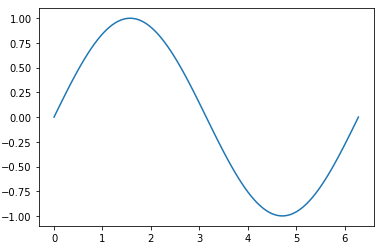
\includegraphics[width=0.4\textwidth]{imgMatPlotLib/grafico1.png}
      \end{figure}
    \end{minipage}
  };
  \node[fancytitle, right=10pt] at (box.north west) {Exemplo de Gráfico com 1 elemento};
\end{tikzpicture}

%------------ Gráfico com vários elementos ---------------------
\begin{tikzpicture}
  \node [mybox] (box){%
	\begin{minipage}{0.3\textwidth} \vspace{0.5em}
	\codigo{x = np.arange(10) \\
		plt.plot(x, x) \\
		plt.plot(x, 2 * x) \\
		plt.plot(x, 3 * x) \\
		plt.plot(x, 4 * x) \\
		plt.legend(['y = x', 'y = 2x', 'y = 3x', 'y = 4x'], loc='upper left')  \\
		plt.show()} \\[2mm]
	Neste gráfico temos uma amostra de como várias funções podem se combinar.
	\begin{figure}[H]
  	  \centering
   	  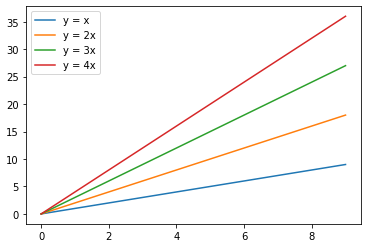
\includegraphics[width=0.5\textwidth]{imgMatPlotLib/grafico2.png}
	  \end{figure}
	\end{minipage}
  };
  \node[fancytitle, right=10pt] at (box.north west) {Exemplo de Gráfico com vários elementos};
\end{tikzpicture}

%------------ Gráfico com vários elementos ---------------------
\begin{tikzpicture}
  \node [mybox] (box){%
	\begin{minipage}{0.3\textwidth} \vspace{0.5em}
	  \codigo{plt.figure(figsize = [8,7]) \\
        t = np.arange(0,2 * np.pi, 0.1) \\
        x = 16 * np.sin(t) ** 3 \\
        y = 13 * np.cos(t) - 5 * np.cos(2 * t) - 2 * np.cos(3 * t) - np.cos(4 * t) \\
        plt.plot(x,y) \\
        plt.title("Viva Python")}
    \end{minipage}
  };
  \node[fancytitle, right=10pt] at (box.north west) {Tente este exemplo};
\end{tikzpicture}
%------------ Mais de um Gráfico ---------------------
\begin{tikzpicture}
  \node [mybox] (box){%
	\begin{minipage}{0.3\textwidth} \vspace{0.5em}
	  Inserir subgráfico: \\
	  \codigo{plt.subplot(nLin, nCol, indice)} \\[2mm]
	  Por exemplo: \\
	  \codigo{ax1 = plt.subplot(2, 2, 1)} \\[2mm]
	  Retirar a borda: \\
	  \codigo{ax1 = plt.subplot(221, frameon=False)} \\[2mm]
	  Adicionar o subgráfico a figura: \\
	  \codigo{plt.subplot(ax1)} \\[2mm]
	  Excluir o subgráfico da figura: \\
	  \codigo{plt.delaxes(ax1)}
	\end{minipage}
  };
  \node[fancytitle, right=10pt] at (box.north west) {MatPlotLib - SubGráficos na Figura};
\end{tikzpicture}

%------------ Exemplo Gráfico com vários elementos ---------------------
\begin{tikzpicture}
  \node [mybox] (box){%
    \begin{minipage}{0.3\textwidth} \vspace{0.5em}
      \codigo{xvals = np.arange(0, 100, 1) \\
        r2 = np.sqrt(xvals) \\
        r3 = np.cbrt(xvals) \\
        ax1 = plt.subplot(121) \\
        ax1.plot(xvals, r2) \\
        plt.subplot(ax1) \\
        ax2 = plt.subplot(122) \\
        ax2.plot(xvals, r3) \\
        plt.suptitle('Comparação entre Raizes') \\
        plt.subplot(ax2) \\
        plt.show()}
      \begin{figure}[H]
        \centering
	    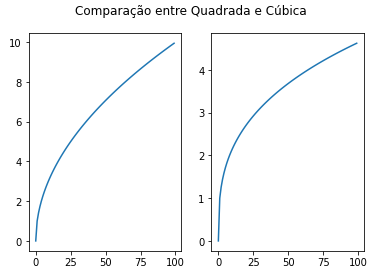
\includegraphics[width=0.6\textwidth]{imgMatPlotLib/grafico3.png}
	  \end{figure}
	  Ou com \underline{axes}: \\
      \codigo{fig, axes = plt.subplots(1, 2, figsize=(10,4)) \\
      	axes[0].plot(xvals, r2) \\
      	axes[0].set\_title("Quadrada") \\
      	axes[1].plot(xvals, r3) \\
      	axes[1].set\_title("Cúbica")}
    \end{minipage}
  };
  \node[fancytitle, right=10pt] at (box.north west) {Exemplo de 2 SubGráficos};
\end{tikzpicture}

\end{multicols*}
\end{document}